% Standard Article Definition
\documentclass[]{article}

% Page Formatting
\usepackage[margin=1in]{geometry}
\setlength\parindent{0pt}

% Graphics
\usepackage{graphicx}

% Math Packages
\usepackage{physics}
\usepackage{amsmath, amsfonts, amssymb, amsthm}
\usepackage{mathtools}

% Extra Packages
\usepackage{pdfpages}
\usepackage{hyperref}
% \usepackage{listings}

% Section Heading Settings
\usepackage{enumitem}
% \renewcommand{\theenumi}{\alph{enumi}}
\renewcommand*{\thesection}{Problem \arabic{section}}
\renewcommand*{\thesubsection}{\alph{subsection})}
\renewcommand*{\thesubsubsection}{}%\quad \quad \roman{subsubsection})}

\newcommand{\Problem}{\subsubsection*{\textbf{PROBLEM:}}}
\newcommand{\Solution}{\subsubsection*{\textbf{SOLUTION:}}}
\newcommand{\Preliminaries}{\subsubsection*{\textbf{PRELIMINARIES:}}}

%Custom Commands
\newcommand{\N}{\mathbb{N}}
\newcommand{\Z}{\mathbb{Z}}
\newcommand{\Q}{\mathbb{Q}}
\newcommand{\R}{\mathbb{R}}
\newcommand{\C}{\mathbb{C}}

\newcommand{\Rel}{\mathcal{R}}

% \newcommand{\toI}{\xrightarrow{\textsf{\tiny I}}}
% \newcommand{\toS}{\xrightarrow{\textsf{\tiny S}}}
% \newcommand{\toB}{\xrightarrow{\textsf{\tiny B}}}

\newcommand{\divisible}{ \ \vdots \ }
\newcommand{\st}{\ : \ }

% Theorem Definition
\newtheorem{definition}{Definition}
\newtheorem{assumption}{Assumption}
\newtheorem{theorem}{Theorem}
\newtheorem{lemma}{Lemma}
\newtheorem{proposition}{Proposition}
% \newtheorem{example}{Example}
% \newtheorem{counterExample}{Counter Example}


%opening
\title{MATH 6301 Real Analysis I \\ Homework 2}
\author{Jonas Wagner\\ jonas.wagner@utdallas.edu}
\date{2022, September 15\textsuperscript{th}}

\begin{document}

\maketitle

\tableofcontents

\includepdf[pages={2}]{math6301a2-2022.pdf}

% Problem 1 ----------------------------------------------
\newpage
\section{}
\Problem
Given two metric spaces $(X,d)$ and $(Y,p)$, $a \in X$, and a function $f \st X \backslash \{a\} \to Y$.
We denote by $A_a(f)$ the set of all accumulated values of $f$ at $a$.
Show that $A_a(f)$ is a closed set.

\Solution






% Problem 2 ----------------------------------------------
\newpage
\section{}
\Problem
Assume that $(X,d)$ is a metric space, $a \in X$ and $f \st X \backslash \{a\} \to \R$ is a function.
Put for $\delta > 0$ \[
    C_\delta(a) \coloneqq \{x \in X \st 0 < d(x,a) < \delta\}
\] Show that \[
    \limsup_{x \to a} = \inf_{\delta > 0} \sup_{x \in C_\delta(a)} f(x)
\]\[
    \liminf_{x \to a} = \sup_{\delta > 0} \inf_{x \in C_\delta(a)} f(x)
\]

\Solution









% Problem 3 ----------------------------------------------
\newpage
\section{}
Given a metric space $(X,d)$, $a \in X$, and a function $f \st X \backslash \{a\} \to \R$ such that $A_a(f) \neq \emptyset$ is also bounded. 

\subsection{}
\Problem
Show that $\limsup_{x \to a} f(x) < \alpha$ for some $\alpha \in \R$ iff \[
    \exists_{\delta>0} \exists_{\overline{\alpha}< \alpha} \forall_{x \in X} 0 < d(x,a) < \delta \implies f(x) \leq \overline{\alpha}
\]
\Solution


\subsection{}
\Problem
Show that $\liminf_{x \to a} f(x) > \alpha$ for some $\alpha \in \R$ iff \[
    \exists_{\delta>0} \exists_{\overline{\alpha} > \alpha} \forall_{x \in X} 0 < d(x,a) < \delta \implies f(x) \geq \overline{\alpha}
\]
\Solution






\subsection{}
\Problem
Show that $\limsup_{x \to a} f(x) \leq \alpha$ for some $\alpha \in \R$ iff \[
    \forall_{\alpha' > \alpha} \exists_{\delta>0} \forall_{x \in X} 0 < d(x,a) < \delta \implies f(x) \leq \alpha'
\]
\Solution






\subsection{}
\Problem
Show that $\liminf_{x \to a} f(x) \leq \alpha$ for some $\alpha \in \R$ iff \[
    \forall_{\alpha' < \alpha} \exists_{\delta>0} \forall_{x \in X}  0 < d(x,a) < \delta \implies f(x) \geq \alpha'
\]
\Solution


% Problem 4 ----------------------------------------------
\newpage
\section{}
\Problem
Given two metric spaces $(X,d)$ and $(Y,p$), $a \in X$ and a function $f \st X \to Y$.
Show that $f$ is continuous iff \[
    A_\alpha(f) = \{f(a)\}
\]
\Solution




% Problem 5 ----------------------------------------------
\newpage
\section{}
Denote by $\overline{\mathbb{R}}$ the ordered set of real numbers $\{-\infty\} \cup \R \cup \{\infty\}$ and define the function $\phi \st \overline{\mathbb{R}} \to \R$ by \[
    \phi(x) = \begin{cases}
        \text{arctan}(x) & x \in \R\\
        \pm \frac{\pi}{2} & x = \pm \infty
    \end{cases}
\] and the function $d \st \overline{\R} \cross \overline{\R} \to \R$ by \[
    d(x,y) \coloneqq \abs{\phi(x) - \phi(y)}
\]

\subsection{}
\Problem
Show that the function $d$ is a metric on $\overline{\R}$.
\Solution


\subsection{}
\Problem
Show that the topology $\mathcal{T}$ induced by the metric $d$ on $\overline{\R}$, restricted to $\R$, coincide with the usual topology on $\R$.
\Solution


% \subsection{}
% \Problem
% Show that $x \in A \iff d(x,A) = 0$.

% \Solution
% \begin{proposition}
%     $x \in A \iff d(x,A) = 0$
% \end{proposition}
% \begin{proof}
%     First we look at $\implies$,\[
%         x \in A \implies \exists d(x,a) \st a \in A = 0 \implies \inf\{0,\dots\} = 0 \implies d(x,A) = \inf\{d(x,a) \st a \in A\} = 0
%     \] Next we look at $\impliedby$, \[
%         d(x,A) = \inf\{d(x,a) \st a \in A\} = 0 \implies \exists_{\{x_n\} \subset A} \st \lim_{n\to \infty} d(x,a) = 0 \implies x \in A
%     \]
% \end{proof}

% \subsection{}
% \Problem
% Show that the function $\Xi_A : X \to \R$ defined by $\Xi_A(x) = d(x,A)$ is continuous on $X$.

% \Preliminaries
% \begin{definition}
%     Let $(X, d_x)$ and $(Y, d_y)$ be metric spaces.
%     A function $f : X \to Y$ is \emph{\underline{continous at point $a \in X$}} iff \[
%         \forall_{\epsilon>0} \exists_{\delta > 0} \forall_{x \in X} d_x(a,x) < \delta \implies d_y(f(x),f(a)) < \epsilon
%     \] $f$ is \emph{\underline{continous}} iff \[
%         \forall_{a \in X} \forall_{\epsilon>0} \exists_{\delta > 0} \forall_{x \in X} d_x(a,x) < \delta \implies d_y(f(x),f(a)) < \epsilon
%     \] Additionally, we have that $f$ is continuous iff the inverse inverse of an open set is open, i.e \[
%         f \ \text{continuous} \ \iff \forall_{\nu \in \tau_Y} f^{-1} (\nu) \in \tau_X
%     \] $f$ is \emph{\underline{univformly continous}} iff \[
%         \forall_{\epsilon>0} \exists_{\delta > 0} \forall_{a \in X} \forall_{x \in X} d_x(a,x) < \delta \implies d_y(f(x),f(a)) < \epsilon
%     \]
% \end{definition}

% \Solution

% \begin{proposition}
%     The function $\Xi_A : X \to \R$ defined by $\Xi_A(x) = d(x,A)$ is continuous on $X$.
% \end{proposition}
% \begin{proof}
%     % Since $A \subset X$ is a closed and non-empty set, 
%     $\Xi_A$ is continuous iff it is continuous at all $a \in X$.
    
%     First, let $a \in A$.
%     Since $x \in A \iff d(x,A) = A$, we have $\forall_{x \in A} \xi_A(x) = 0$ which implies \[
%         \forall_{a \in A} \forall_{\epsilon>0} \exists_{\delta > 0} \forall_{x \in A} d_x(a,x) < \delta \implies d_y(\Xi_A(x) = 0,\Xi_A(a) = 0) = 0 < \epsilon
%     \]

%     Next, let $a \in X \backslash A$.
%     The set $X \backslash A$ is open.
%     Since $\forall_{a \in X \backslash A}$ we have that $d_A(x,a) > 0$, we define $\tau_Y$ as the open set $y > 0$.
%     Since both $\tau_X = X \backslash A$ and $y>0$ are open, we have that \[
%         \forall_{\nu \in \tau_Y} \Xi^{-1} (\nu) \in \tau_X
%     \]

%     Finally, at the boundary of $A$, we have that for $x \notin A$, \[
%         \lim_{a \to A} \Xi_A(a) = 0
%     \] which implies Continuity at the boundary.

%     Therefore, $\Xi_A$ is continuous at all $a \in X$ which means $\Xi_A$ is a continuous function.
% \end{proof}






\end{document}
